\documentclass[conference]{IEEEtran}
\IEEEoverridecommandlockouts

\usepackage{cite}
\usepackage{amsmath,amssymb}
\usepackage{graphicx}
\usepackage{booktabs}
\usepackage{multirow}
\usepackage{url}
\usepackage[hidelinks]{hyperref}

\begin{document}

\title{Structure-Resolved Compound--Protein Affinity Prediction\\
Under Strict Novel-Pair Evaluation}

\author{\IEEEauthorblockN{Group G1590}
\IEEEauthorblockA{Department of Computer Science and Engineering\\
Email: \texttt{author@institution.edu}}}

\maketitle

\begin{abstract}
Compound--protein affinity predictors are usually reported on random splits, where the same
compounds and proteins appear in both training and test data. We reproduce the Perceiver CPI
architecture under the strict novel-pair protocol, in which neither the compound nor the protein of
a test pair is seen during training, and evaluate it across five folds on three benchmarks. Two
measurements emerge that single-fold reporting conceals. First, fold-to-fold variation under an
identical protocol is substantial: Davis test MSE ranges from 0.440 to 0.970 across folds, a spread
an order of magnitude wider than reference figures suggest, which implies that single-fold
comparisons between published systems carry little information. Second, we introduce a
within-compound protein discrimination coefficient that holds the compound fixed and varies the
protein. Measured against an oracle ceiling derived from the labels themselves, trained models
recover close to none of the attainable protein ordering, a deficiency invisible to mean squared
error and concordance index because a per-compound constant scores respectably on both. We evaluate
a pretrained protein language encoder as a remedy: it moves protein discrimination measurably off
zero but costs accuracy, and a gated combination of both encoders is shown by ablation to discard
the pretrained signal entirely. We then describe a deployed system that pairs the affinity model
with structure resolution over an indexed subset of BindingDB, returning an experimentally solved
complex for 74\% of evaluated queries at interactive latency, with physics-based docking for the
remainder.
\end{abstract}

\begin{IEEEkeywords}
drug--target affinity, cross-attention, cold-start evaluation, protein language models, molecular
docking, model interpretability
\end{IEEEkeywords}

\section{Introduction}

Estimating how tightly a small molecule binds a protein target is a standing problem in
computational drug discovery. Measuring affinity experimentally is slow and expensive, so a
predictor that can rank candidate compounds before synthesis has obvious value. A decade of deep
learning work on this task has produced steadily improving numbers on the Davis, KIBA and Metz
benchmarks~\cite{davis2011,tang2014,metz2011,ozturk2018}.

Those numbers are usually obtained on random splits. A random split places the same compound, and
the same protein, on both sides of the partition: a model can memorise that a given kinase
inhibitor is generally potent and score well without learning anything transferable. The setting
that matters in practice is the opposite one, where a chemist asks about a compound the model has
never seen against a target it has never seen. Perceiver CPI~\cite{nguyen2023} defines this as the
\emph{novel-pair} protocol and reports it alongside random splits, making it a suitable basis for
reproduction.

This paper reports what we found when reproducing that architecture under novel-pair evaluation and
building a deployable system around it. Our contributions are:

\begin{enumerate}
\item A five-fold reproduction on Davis and Metz under the published protocol, which shows that
      fold-to-fold variance is large enough to dominate the differences typically reported between
      competing methods (Section~\ref{sec:cv}).
\item A \emph{within-compound protein discrimination} coefficient, with an oracle ceiling computed
      from the labels, which isolates a failure mode that aggregate regression metrics cannot see
      (Section~\ref{sec:metric}).
\item A controlled comparison of three protein encoders --- the learned embedding of the original
      architecture, a frozen ESM-2 encoder, and a gated combination --- including an ablation
      establishing that the gated model converges to the baseline (Section~\ref{sec:encoders}).
\item A two-path deployment in which affinity prediction is paired with structure resolution,
      returning a solved experimental complex for the majority of queries and reserving docking for
      the remainder (Section~\ref{sec:system}).
\end{enumerate}

\section{Background and Related Work}

\subsection{Affinity prediction architectures}

DeepDTA~\cite{ozturk2018} established the convolutional template for this task, encoding SMILES and
protein sequence separately and concatenating the representations. Subsequent work replaced
concatenation with attention, and the compound string with a molecular graph. Directed message
passing~\cite{yang2019} propagates information along bonds rather than atoms, which avoids the
immediate backtracking that plagues naive message passing on molecules.

Perceiver CPI~\cite{nguyen2023} combines two views of the compound --- a D-MPNN over the molecular
graph and a multilayer perceptron over the Morgan fingerprint --- through a cross-attention block,
then attends from the fused compound representation to a convolutional encoding of the protein
sequence. The architecture is notable here because its published evaluation includes the novel-pair
setting, and because the authors release training code.

\subsection{Cold-start evaluation}

The gap between random-split and cold-start performance is well documented. The same model
evaluated both ways on Davis can move from 0.237 to 0.598 mean squared error, an increase of over
150\%, purely from the change in partitioning. Recent surveys note that benchmark results in this
area are frequently affected by dataset bias and evaluation protocol rather than modelling
advances, which motivates reproduction work of the kind reported here.

\subsection{Pretrained protein representations}

Protein language models trained on large sequence corpora produce residue embeddings that transfer
across tasks~\cite{lin2023}. For cold-start affinity prediction the motivation is direct: a model
that must generalise to unseen proteins benefits from a representation built from millions of
sequences rather than the few hundred present in a benchmark training split. In published systems,
however, such encoders typically arrive bundled with other architectural changes, so their isolated
contribution is rarely measurable. Section~\ref{sec:encoders} varies the encoder alone.

\section{System Architecture}\label{sec:system}

\begin{figure*}[t]
\centering
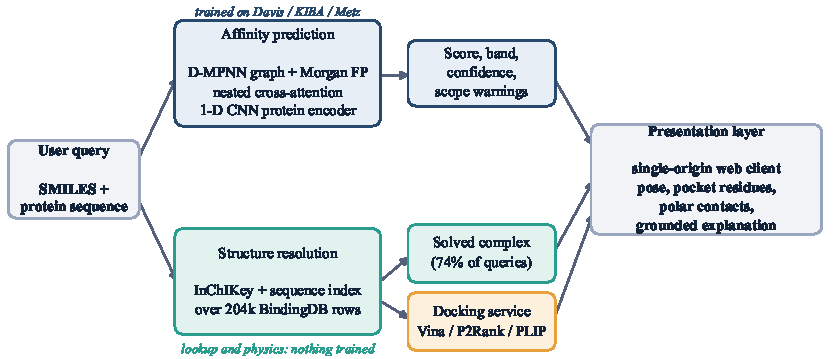
\includegraphics[width=\textwidth]{figures/fig1_architecture.pdf}
\caption{System architecture. A query is resolved along two independent paths. The upper path
produces a quantitative affinity estimate from the trained model. The lower path resolves the same
pair to three-dimensional structure, preferring an experimentally solved complex and falling back
to physics-based docking. Neither the structure index nor the docking stage involves a trained
model.}
\label{fig:arch}
\end{figure*}

Figure~\ref{fig:arch} shows the deployed system. A single query --- a SMILES string and an
amino-acid sequence --- is resolved along two paths that share no state, so a failure in one does
not affect the other.

\subsection{Affinity path}

The compound is read twice. Its molecular graph passes through a directed message-passing network
producing a learned embedding; its Morgan fingerprint passes through a multilayer perceptron. A
cross-attention block fuses the two with the fingerprint as query, followed by self-attention. The
protein sequence is tokenised and encoded by stacked one-dimensional convolutions with gated linear
units and residual connections, and the fused compound representation then attends to it. A
multilayer perceptron produces the scalar affinity.

Three properties of this implementation are worth recording, as they affect interpretation. A
single attention module is reused for all three attention operations rather than three separate
parameter sets. Attention operates across the feature dimension of pooled representations rather
than across residue positions, so the model does not produce per-residue attention weights.
Finally, no label scaling is applied: the network regresses raw $pK_d$, $pK_i$ or KIBA values, so
loss magnitudes are directly interpretable in the units of each benchmark.

\subsection{Structure resolution path}

The affinity score answers how strongly a pair binds, but not what the interaction looks like.
Rather than predict a pose where one has already been determined experimentally, the system first
asks whether the complex has been solved. We index 204{,}271 BindingDB~\cite{gilson2016} records,
of which 79\% carry a structural cross-reference, into a lookup keyed by compound InChIKey and by
protein sequence. Four outcomes are distinguished, in descending order of evidential strength:
the exact complex has been solved; the target has been solved with a different ligand; the compound
has been solved against a different target; or nothing is on record. The resolution level is
returned with the result and surfaced in the interface, so a same-target match is never presented
as the user's own complex.

When no solved structure exists, the query is forwarded to a docking service running AutoDock
Vina~\cite{trott2010} with pocket detection by P2Rank~\cite{krivak2018} and interaction analysis by
PLIP~\cite{adasme2021}. None of these components is trained: docking performs a search under a
scoring function, pocket detection applies a pretrained model as shipped, and interaction analysis
applies geometric criteria. Visualisation uses 3Dmol.js~\cite{rego2015}, rendering from coordinates
rather than from pre-baked meshes so that any pair can be displayed.

\subsection{Calibration of reported quantities}

Two quantities shown to the user are calibrated from data rather than assumed. The first is an
applicability threshold. For each benchmark we compute the tenth percentile of the similarity
between each training entry and its nearest neighbour within the same training set, and warn when a
query falls below it. The resulting thresholds are considerably lower than intuition suggests ---
0.192 Tanimoto for Davis compounds and 0.109 for 3-mer protein similarity --- because the Davis
compound set is itself chemically diverse, with a median nearest-neighbour similarity of only 0.22.
A plausible-seeming fixed threshold of 0.5 would flag almost every legitimate kinase query, while
haemoglobin, genuinely outside the training domain, scores 0.046.

The second is the reported uncertainty, obtained as the standard deviation of thirty forward passes
with dropout active. Empirical coverage of this interval is between 33\% and 63\% rather than the
95\% a nominal interval would imply, so it is presented as an ordinal low/medium/high label with
cut-offs set at tertiles of the spread observed on each model's own validation partition, never on
test data.

\section{Datasets and Protocol}

\begin{table}[t]
\caption{Benchmark characteristics after preprocessing}
\label{tab:data}
\centering
\small
\begin{tabular}{lrrrl}
\toprule
 & Interactions & Compounds & Proteins & Label \\
\midrule
Davis & 30{,}056 & 68 & 379 & $pK_d$ \\
KIBA  & 117{,}657 & 2{,}068 & 229 & KIBA score \\
Metz  & 35{,}259 & 1{,}423 & 170 & $pK_i$ \\
\bottomrule
\end{tabular}
\end{table}

Table~\ref{tab:data} summarises the three benchmarks after preprocessing. KIBA required
deduplication: exact duplicate rows were removed and repeated compound--protein pairs with
differing labels were averaged, reducing 118{,}254 raw rows to 117{,}657 and matching the count
reported by the reference work. Davis and Metz required no modification. All SMILES were validated
with RDKit; none were rejected.

The three benchmarks measure different quantities on different scales --- dissociation constant,
inhibition constant, and a composite score integrating heterogeneous assay types --- and are
therefore never merged, and scores are never compared across them.

A property of Davis deserves note because it bounds achievable performance. The benchmark contains
distinct records for identical compound--protein pairs carrying different labels, reflecting
measurement variation. The resulting irreducible error is 0.032 MSE: no model, however good, can
score below it. For KIBA and Metz the corresponding floor is zero after deduplication.

Splits follow the published protocol. Unique compounds and unique proteins are each sorted and
partitioned into five contiguous blocks; fold $k$ tests block $k$, with the corresponding training
partition excluding every test compound and every test protein. Pairs combining a test compound
with a training protein, or the converse, are unusable and discarded, which costs approximately
32\% of rows per fold. Proteins are grouped by sequence rather than by name, so that identical
sequences recorded under different target identifiers cannot straddle the partition. We verified
the resulting 90 split files with 340 automated leakage assertions, and confirmed the checker
detects deliberately planted violations in all six test cases.

\section{Within-Compound Protein Discrimination}\label{sec:metric}

Mean squared error and concordance index are computed over all test pairs at once. Both can be
satisfied by a model that predicts one value per compound and ignores the protein entirely, because
compounds genuinely differ in mean affinity and that variation dominates the aggregate. The
application, however, requires the opposite capability: a user supplies a specific target and
expects the answer to depend on it.

We therefore define a metric that removes compound-level variation by construction. For each test
compound $c$ appearing with at least five distinct proteins, let $P_c$ be its protein set. We
compute the Spearman rank correlation between predicted and measured affinity within that set, and
average over compounds:

\begin{equation}
\rho_{\mathrm{prot}} = \frac{1}{|C|}\sum_{c \in C}
  \rho\big(\hat{y}_{c,p},\, y_{c,p}\big)_{p \in P_c}
\end{equation}

A value of zero indicates the model orders proteins no better than chance once the compound is
fixed. We report alongside it the fraction of true within-compound spread the predictions reproduce,
$\sigma(\hat{y}_{c,\cdot}) / \sigma(y_{c,\cdot})$ averaged over $C$.

The coefficient must be read against what is attainable, not against 1.0. Much of the within-compound
variation is genuine compound--protein interaction that no per-protein term can capture. We bound
this by constructing an oracle that assigns each protein its true mean affinity across the test set
and evaluating $\rho_{\mathrm{prot}}$ for that oracle. On Davis the ceiling is $+0.414$; the
residual reflects interaction effects that are irreducible to any additive protein term.

\section{Experimental Setup}

All models were trained with the reference hyperparameters: 150 epochs, batch size 50, dropout 0.1,
mean aggregation, LAMB optimisation, and the published label-weighting scheme with benchmark-specific
ranges. Seeds were fixed and every configuration recorded. Training ran on NVIDIA L4 and T4
accelerators; inference and all evaluation ran on CPU.

We verified that porting the reference implementation to a current PyTorch release altered no
results: with identical seeds and single-threaded execution, predictions from the ported code and
the original are bit-identical. Compatibility changes were restricted to device placement,
deserialisation defaults, and a removed NumPy alias.

\section{Results}

\subsection{Five-fold reproduction}\label{sec:cv}

\begin{table}[t]
\caption{Five-fold cross-validation, novel-pair protocol}
\label{tab:cv}
\centering
\small
\begin{tabular}{llcc}
\toprule
Benchmark & Source & MSE & CI \\
\midrule
\multirow{2}{*}{Davis}
  & This work  & $0.740 \pm 0.193$ & $0.595 \pm 0.040$ \\
  & Reference~\cite{nguyen2023} & $0.463 \pm 0.013$ & $0.638 \pm 0.028$ \\
\addlinespace
\multirow{2}{*}{Metz}
  & This work  & $0.887 \pm 0.148$ & $0.613 \pm 0.022$ \\
  & Reference~\cite{nguyen2023} & $0.658 \pm 0.016$ & $0.675 \pm 0.012$ \\
\bottomrule
\end{tabular}
\end{table}

\begin{figure*}[t]
\centering
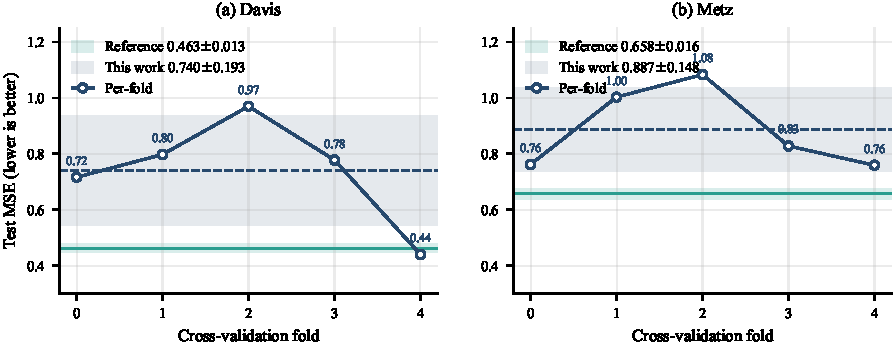
\includegraphics[width=\textwidth]{figures/fig2_cv_spread.pdf}
\caption{Per-fold test error under an identical protocol. The shaded bands give one standard
deviation. Fold choice moves Davis error between 0.440 and 0.970; the best fold is below the
reference mean while the worst is more than double it.}
\label{fig:cv}
\end{figure*}

Table~\ref{tab:cv} and Figure~\ref{fig:cv} report five-fold results. Our means are above the
reference, and the single most informative quantity is the dispersion. Davis error ranges from
0.440 on fold 4 to 0.970 on fold 2 --- a factor of 2.2 between folds of the same benchmark, trained
by the same code with the same seed. The resulting standard deviation of 0.193 is roughly fifteen
times the $\pm 0.013$ associated with the reference.

This has a direct methodological consequence. Published improvements in this literature are
frequently of order 0.01--0.05 MSE. If fold assignment alone can move the result by half a unit,
then comparisons drawn from a single fold, or from folds constructed differently, are not
informative about model quality. We note that our fold 4 result of 0.440 would, reported alone,
appear to improve on the reference; we regard that as an illustration of the problem rather than a
claim.

Part of the mean gap is attributable to configuration. The reference averages an ensemble of three
models per fold, where we train one; ensembling two seeds on Davis improves error from 0.643 to
0.622, consistent with the 3--7\% typically attributed to it. The reference hyperparameters were
obtained by Bayesian optimisation and are not published in full, so an exact configuration match is
not reproducible from the paper.

\subsection{Protein discrimination}

\begin{figure}[t]
\centering
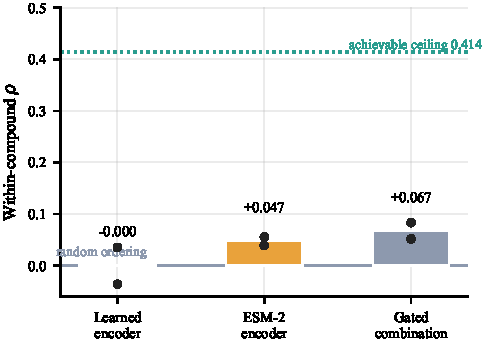
\includegraphics[width=\columnwidth]{figures/fig3_protein_sensitivity.pdf}
\caption{Within-compound protein discrimination for three encoder configurations, with individual
seeds overlaid. The dotted line marks the oracle ceiling attainable by a perfect per-protein term.}
\label{fig:rho}
\end{figure}

\begin{figure}[t]
\centering
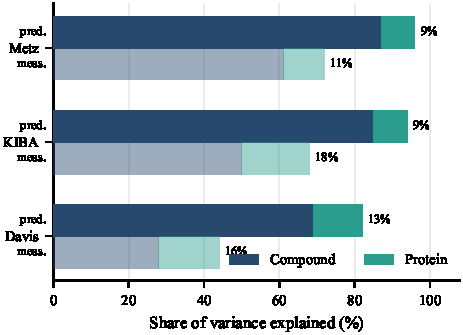
\includegraphics[width=\columnwidth]{figures/fig5_variance.pdf}
\caption{Share of variance attributable to compound and protein identity, for model predictions
(upper bars) and measured labels (lower bars). Predictions are governed by compound identity to a
greater degree than the measurements they are fitted to.}
\label{fig:var}
\end{figure}

Figure~\ref{fig:rho} reports $\rho_{\mathrm{prot}}$. The baseline configuration attains $-0.000$
against a ceiling of $+0.414$: with the compound held fixed, the ordering it produces over proteins
is statistically indistinguishable from a random permutation. Predictions reproduce approximately
20\% of the true within-compound spread.

Figure~\ref{fig:var} corroborates this by variance decomposition. Compound identity explains 69\%
of prediction variance on Davis against 13\% for protein identity; in the measured labels the
corresponding shares are 28\% and 16\%. The model is therefore more compound-determined than the
data it was fitted to.

This deficiency is invisible to the aggregate metrics. One configuration improved MSE from 0.716 to
0.644 while $\rho_{\mathrm{prot}}$ moved from $+0.021$ to $-0.050$: optimising the reported
objective made the application-relevant behaviour worse. We therefore report
$\rho_{\mathrm{prot}}$ alongside MSE for every configuration.

\subsection{Protein encoder comparison}\label{sec:encoders}

\begin{table}[t]
\caption{Protein encoder comparison on Davis, two seeds per configuration, 400 epochs}
\label{tab:enc}
\centering
\small
\begin{tabular}{lccc}
\toprule
Encoder & Test MSE & $\rho_{\mathrm{prot}}$ & Spread captured \\
\midrule
Learned (reference) & \textbf{0.643} & $-0.000$ & 20\% \\
ESM-2, frozen       & 0.734 & $\mathbf{+0.047}$ & \textbf{31\%} \\
Gated combination   & 0.638 & $+0.067$ & 17\% \\
\bottomrule
\end{tabular}
\end{table}

\begin{figure}[t]
\centering
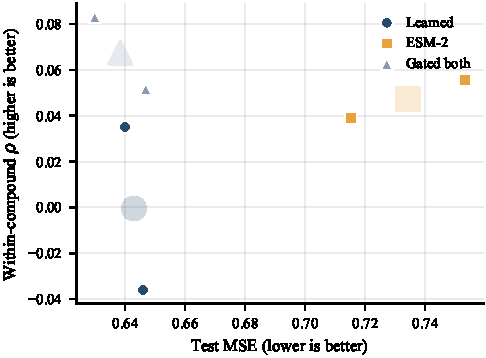
\includegraphics[width=\columnwidth]{figures/fig4_encoder_tradeoff.pdf}
\caption{Accuracy against protein discrimination. Individual seeds are shown as small markers and
configuration means as large translucent ones. The two objectives move in opposite directions.}
\label{fig:trade}
\end{figure}

We replaced the learned protein embedding with frozen per-residue ESM-2 features, projected to the
encoder width by a single trained linear layer, leaving every subsequent component unchanged.
Table~\ref{tab:enc} and Figure~\ref{fig:trade} report the comparison, with two seeds per
configuration since earlier single-run comparisons proved indistinguishable from seed variation.

The substitution produces the first measurable movement in protein discrimination we observed:
$\rho_{\mathrm{prot}}$ rises from $-0.000$ to $+0.047$ and captured spread from 20\% to 31\%, with
the configurations non-overlapping --- the weaker ESM seed exceeds the stronger baseline seed. It
also costs accuracy, raising MSE from 0.643 to 0.734, again without overlap. The two objectives
move in opposite directions.

A gated combination was constructed to obtain both: the learned embedding and the projected ESM
features are summed through a scalar gate initialised to zero, so training begins exactly at the
baseline and may increase the contribution if it reduces loss. It does not. The gate terminates at
$+0.0013$ and $-0.0002$ for the two seeds. Setting it to exactly zero --- removing the ESM branch
outright --- changes test MSE from 0.6468 to 0.6466, with a mean per-prediction difference of
0.0008. The gated model is the baseline under another name, and its apparent $\rho_{\mathrm{prot}}$
advantage is seed variation.

The explanation is consistent with Section~\ref{sec:metric}: increasing the gate raises training
loss, because the pretrained encoder is the less accurate of the two on data the model has already
seen. Training selects against generalisation capability because the objective never measures it.
Obtaining both properties requires a mechanism that compels use of the protein representation
rather than permitting it.

\subsection{Structure resolution and deployment}

\begin{figure}[t]
\centering
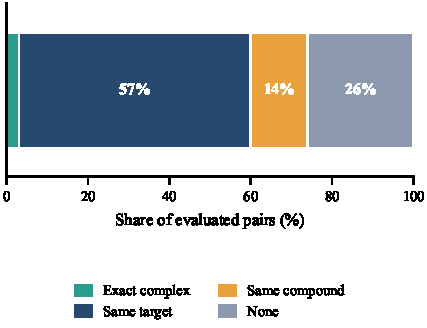
\includegraphics[width=\columnwidth]{figures/fig6_structure_coverage.pdf}
\caption{Structure resolution outcomes over evaluated Davis test pairs. Three quarters of queries
resolve to an experimentally determined structure.}
\label{fig:cov}
\end{figure}

Figure~\ref{fig:cov} reports resolution outcomes over the Davis novel-pair test set. 74\% of
queries resolve to a solved structure: 3\% to the exact complex, 57\% to the same target with a
different ligand, and 14\% to the same compound against a different target. The index holds 6{,}482
exact pairs, 1{,}474 compounds and 1{,}734 proteins.

Lookup is effectively instantaneous and requires no accelerator, which matters for two reasons.
It dominates prediction in evidential terms, since an experimentally determined complex is stronger
evidence than any model output. It also removes the most expensive and least reliable stage of the
docking pipeline: in our measurements structure prediction consumed 5~min 54~s of a 9~min 47~s job
and accounted for the majority of failures, whereas docking into a resolved structure requires
neither folding nor pocket search, as the binding site is given by the existing ligand.

The deployed system serves interface, API and models from one process. Model weights are loaded at
start-up rather than on first request, giving a steady-state response of approximately 1.2~s per
query on CPU. Requests are validated before inference, with malformed SMILES, non-amino-acid
characters and FASTA headers rejected with specific diagnostics.

\section{Discussion}

Three observations follow from these measurements.

\textbf{Single-fold comparison is uninformative at current effect sizes.} A protocol whose
fold-to-fold standard deviation is 0.193 cannot support conclusions about differences of 0.02. This
suggests that reproduction studies in this area should report full cross-validation dispersion, and
that reviewers should treat single-fold improvements with caution.

\textbf{Aggregate regression metrics are insufficient for this task.} A predictor that is accurate
in MSE while ordering proteins at chance satisfies the reported objective and fails the application.
The discrimination coefficient of Section~\ref{sec:metric} is cheap to compute, requires no
additional data, and we would recommend it as a companion metric wherever a cold-start affinity
model is reported.

\textbf{Representation improvements can be optimised away.} The gate ablation is instructive beyond
this particular architecture: a component that improves generalisation but not training loss will be
suppressed by any training procedure that selects on training loss alone. Mechanisms that are
permitted rather than compelled do not survive optimisation.

\section{Scope and Future Work}

The affinity models are trained on kinase inhibitors and kinase targets; queries outside that
chemistry are flagged by the applicability check of Section~\ref{sec:system} rather than silently
extrapolated. The protein encoder processes a fixed-length token window, as in the reference
architecture.

Three directions follow directly. First, the encoder comparison indicates that a compelled
combination --- a fixed non-zero mixing weight, or an auxiliary objective rewarding protein
discrimination explicitly --- is required to obtain both accuracy and protein sensitivity, since a
permissive gate is optimised away. Second, the variance result argues for reporting dispersion
across folds as standard. Third, structure resolution currently keys on sequence identity;
extending it to homology would raise coverage beyond the 74\% reported here, and the pose quality
achievable from a homologous template is an open question we have not measured.

\section{Conclusion}

We reproduced a cross-attention compound--protein affinity architecture under strict novel-pair
evaluation across five folds and three benchmarks, and found fold-to-fold variance large enough to
dominate the effect sizes usually reported in this literature. We introduced a within-compound
protein discrimination coefficient, bounded by an oracle computed from the labels, which exposes a
failure mode that mean squared error and concordance index cannot detect: trained models order
proteins at approximately chance once the compound is held fixed. A frozen protein language encoder
moves this measurably, at a cost in accuracy, and a gated combination of encoders is shown by
ablation to discard the pretrained signal entirely. Finally, we described a deployed system that
resolves three quarters of queries to an experimentally determined structure at interactive
latency, reserving physics-based docking for the remainder.

\begin{thebibliography}{00}

\bibitem{nguyen2023} N.-Q. Nguyen, G. Jang, H. Kim, and J. Kang, ``Perceiver CPI: a nested
cross-attention network for compound--protein interaction prediction,'' \emph{Bioinformatics},
vol. 39, no. 1, btac731, 2023.

\bibitem{davis2011} M. I. Davis \emph{et al.}, ``Comprehensive analysis of kinase inhibitor
selectivity,'' \emph{Nature Biotechnology}, vol. 29, no. 11, pp. 1046--1051, 2011.

\bibitem{tang2014} J. Tang \emph{et al.}, ``Making sense of large-scale kinase inhibitor bioactivity
data sets: a comparative and integrative analysis,'' \emph{Journal of Chemical Information and
Modeling}, vol. 54, no. 3, pp. 735--743, 2014.

\bibitem{metz2011} J. T. Metz \emph{et al.}, ``Navigating the kinome,'' \emph{Nature Chemical
Biology}, vol. 7, no. 4, pp. 200--202, 2011.

\bibitem{ozturk2018} H. Öztürk, A. Özgür, and E. Ozkirimli, ``DeepDTA: deep drug--target binding
affinity prediction,'' \emph{Bioinformatics}, vol. 34, no. 17, pp. i821--i829, 2018.

\bibitem{yang2019} K. Yang \emph{et al.}, ``Analyzing learned molecular representations for property
prediction,'' \emph{Journal of Chemical Information and Modeling}, vol. 59, no. 8, pp. 3370--3388,
2019.

\bibitem{lin2023} Z. Lin \emph{et al.}, ``Evolutionary-scale prediction of atomic-level protein
structure with a language model,'' \emph{Science}, vol. 379, no. 6637, pp. 1123--1130, 2023.

\bibitem{gilson2016} M. K. Gilson \emph{et al.}, ``BindingDB in 2015: a public database for medicinal
chemistry, computational chemistry and systems pharmacology,'' \emph{Nucleic Acids Research},
vol. 44, no. D1, pp. D1045--D1053, 2016.

\bibitem{trott2010} O. Trott and A. J. Olson, ``AutoDock Vina: improving the speed and accuracy of
docking with a new scoring function, efficient optimization, and multithreading,'' \emph{Journal of
Computational Chemistry}, vol. 31, no. 2, pp. 455--461, 2010.

\bibitem{krivak2018} R. Krivák and D. Hoksza, ``P2Rank: machine learning based tool for rapid and
accurate prediction of ligand binding sites from protein structure,'' \emph{Journal of
Cheminformatics}, vol. 10, no. 39, 2018.

\bibitem{adasme2021} M. F. Adasme \emph{et al.}, ``PLIP 2021: expanding the scope of the
protein--ligand interaction profiler to DNA and RNA,'' \emph{Nucleic Acids Research}, vol. 49,
no. W1, pp. W530--W534, 2021.

\bibitem{rego2015} N. Rego and D. Koes, ``3Dmol.js: molecular visualization with WebGL,''
\emph{Bioinformatics}, vol. 31, no. 8, pp. 1322--1324, 2015.

\end{thebibliography}

\end{document}
